\chapter{Thesis Contribution}
\label{ch:contribution}

\section{Conceptual Model}
Figure \ref{fig:concept} shows the conceptual model of the system in the form of a block diagram.

\begin{figure}[h]
    \centering
    \includegraphics[scale=0.4]{images/Conceptual_Model.png}
    \caption{Conceptual Model}
    \label{fig:concept}
\end{figure}

The system is divided into a physical and a virtual system, which is linked by the Linux PC hosting the \acrshort{CoAP} fileserver. The physical system is replicated in the virtual system and tracked by reading the process updates from the fileserver. Similarly, the physical system is updated by accessing the update files from the fileserver and flashing onto each module simultaneously.

\section{Implementation}
This section elaborates on the hardware system, the software configuration, and the interfaces between them to provide a detailed description of the system which has been set up as a proof of concept for the theory described in Chapter \ref{ch:introduction}. 

\subsection{Hardware Setup}
Factory modules such as conveyors (Figure \ref{fig:tt_con}), sliders (Figure \ref{fig:slider}), and turntables (Figure \ref{fig:tt_con}) which are available in the Factory Planning Laboratory of the \acrfull{ILM} department at Otto-von-Guericke University, are utilized for experimentation purposes of this thesis.

\begin{figure}
    \centering
    \includegraphics[scale=0.5]{images/TT_Conv.png}
    \caption{Conveyor and Turntable \cite{Karri_2021}}
    \label{fig:tt_con}
\end{figure}

\begin{figure}
    \centering
    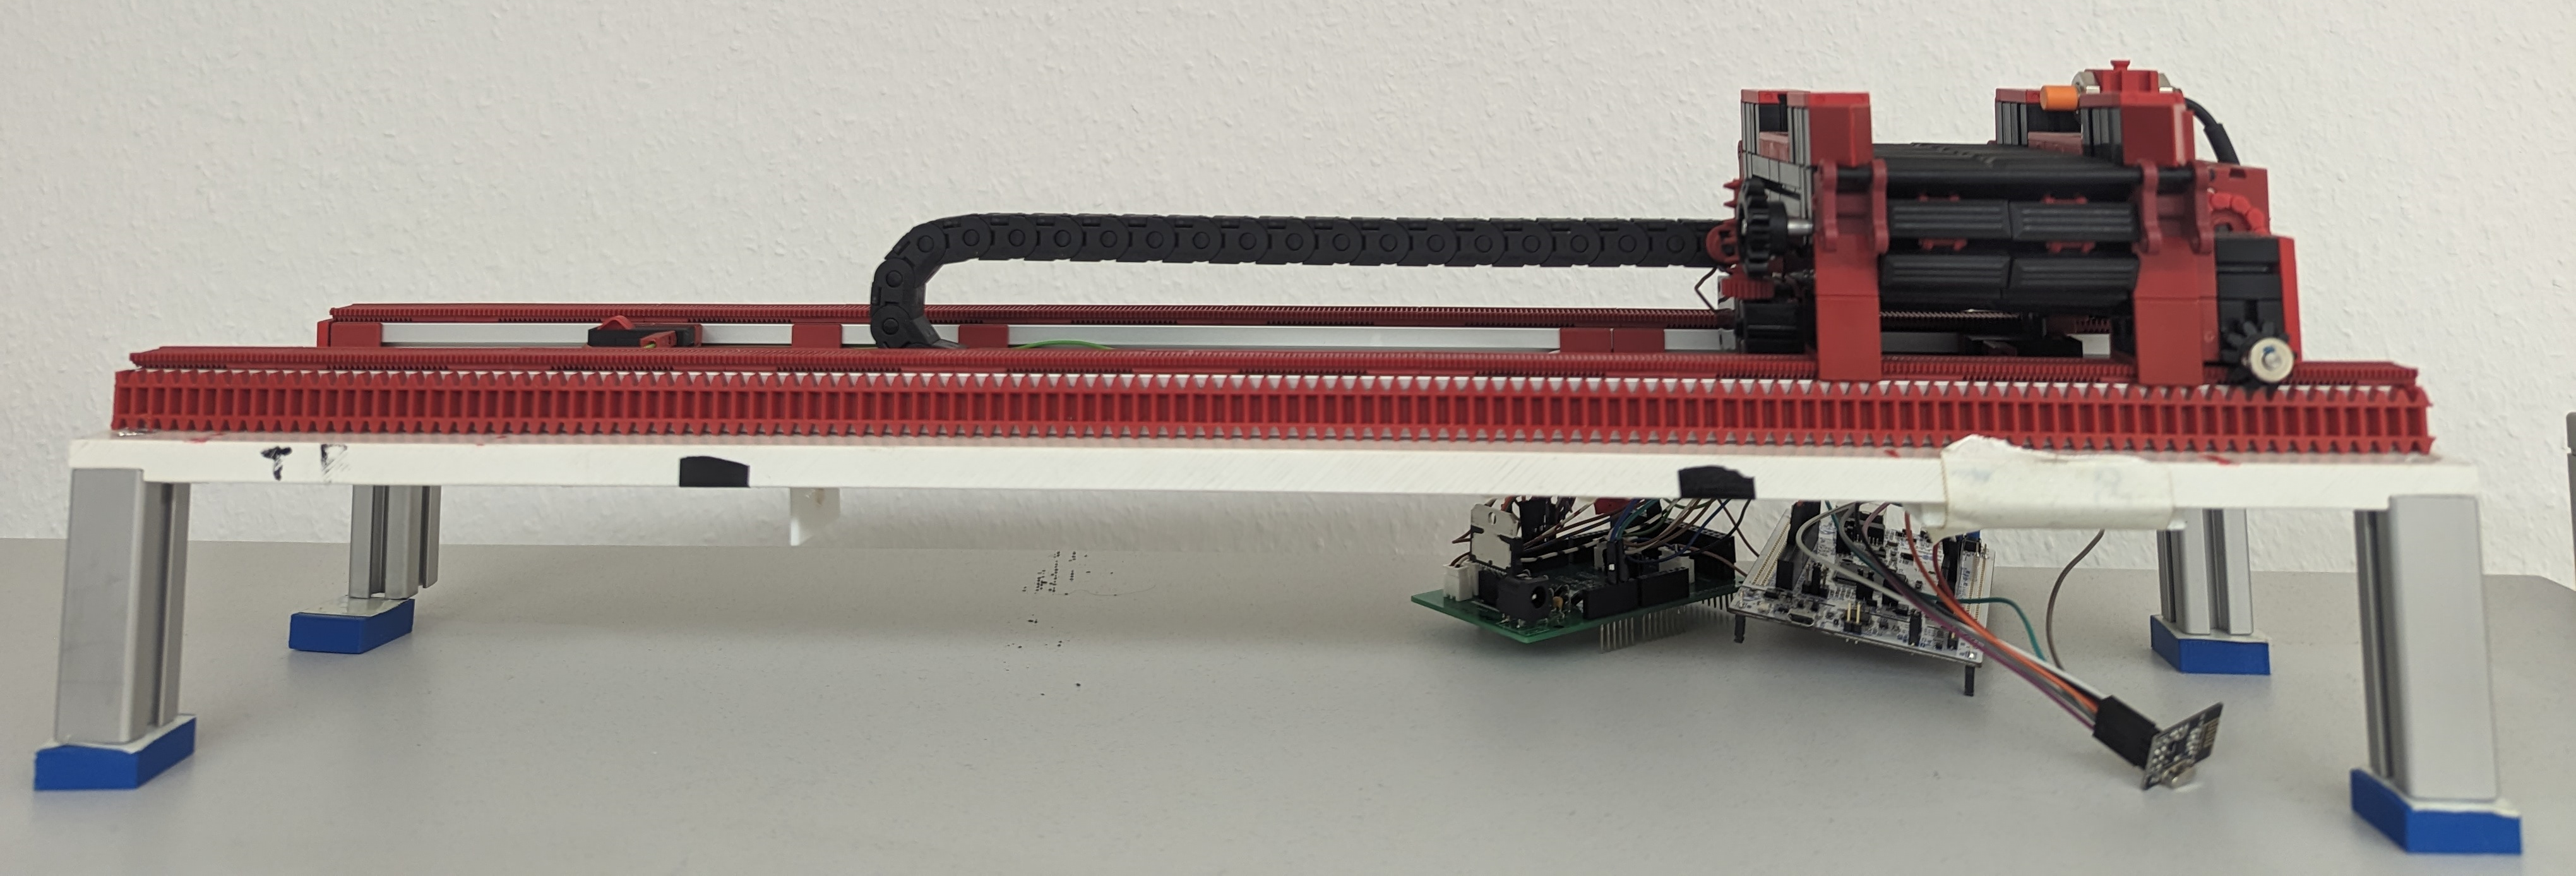
\includegraphics[scale=0.12]{images/Slider.png}
    \caption{Slider}
    \label{fig:slider}
\end{figure}

After careful research on different \acrshort{MCU} based on the requirements of this work, ARM-based STM32F767ZI Nucleo-144 mbed-enabled development boards (Figure \ref{fig:nucleo}) are selected as the controllers for these factory modules. Some of the features of these boards include a 32-bit ARM-based STM32 controller, up to 512kBytes of SRAM, up to 216MHz of operating frequency, and a 144-pin layout with multiple application-specific hardware add-on capabilities. The STM32 boards boast an impressive number of peripherals when compared to boards like the PIC32, and also can be much more reliable when running power-demanding applications.
\begin{figure}[h]
    \centering
    \includegraphics[scale=0.4]{images/NucleoBoard.png}
    \caption{Nucleo-F767ZI Microcontroller Board \cite{ARM_2017}}
    \label{fig:nucleo}
\end{figure}

One of the drawbacks of the Nucleo F767ZI board is the lack of wireless connectivity, as there is only an ethernet port to connect to a network. The use of an ESP32 board can cover this shortcoming by running a border router application on it and connecting it to the Nucleo board using UART, as shown in Figure \ref{fig:esp_con}.
\begin{figure}
    \centering
    \includegraphics{images/ESP_Conn.png}
    \caption{Nucleo-F767ZI - ESP32 Connections}
    \label{fig:esp_con}
\end{figure}


\begin{figure}
    \centering
    \includegraphics[scale=0.7, angle=270]{images/LiFi.png}
    \caption{Nucleo-F767ZI - LiFi Connections}
    \label{fig:lifi}
\end{figure}

The modules communicate with each other using \acrshort{LiFi} and RF communication. \acrshort{LiFi} communication is achieved using the \acrshort{LiFi} protocol\cite{mukku2019integration}, with each module containing an LED and an LDR as shown in Figure \ref{fig:lifi}. The LED can emit light pulses at a preset frequency while the LDR can convert these pulses to an analog value, which can be later converted using an ADC to a digital value to be processed by the microcontroller.
Meanwhile, RF communication is achieved by nRF24L01+ transceiver modules which can be seen in Figure \ref{fig:nrf}. Each nRF24L01+ can be configured either as a transmitter or a receiver. Each module has 6 communication channels, so each transmitter module can send data simultaneously to 6 different receiver modules. RIOT OS contains well-documented drivers for nRF24L01+ including test applications, and hence it makes a perfect addition to this system.

\begin{figure}
    \centering
    \includegraphics[scale=0.7, angle=270]{images/Nrf.png}
    \caption{Nucleo-F767ZI - NRF24L01+ Transceiver Connections}
    \label{fig:nrf}
\end{figure}

\subsection{Software Setup}

RIOT OS is used as the operating system for its advantages in multi-threaded operation, well-defined \acrshort{OTA} update mechanism, and real-time updates to the server. \acrshort{CoAP} is used as the communication protocol as it has many advantages such as being lightweight, UDP-based, and thoroughly implemented and documented in the RIOT OS architecture. C programming language is used to program the factory modules on top of the RIOT kernel.

Unity3D is used as the platform to develop a visual interface for the digital twin. The 3D models of the factory modules have been designed in an open-source modeling software called Blender. The background code is written in C\# language which includes the programs to create a network, create the necessary interfaces for communicating with the hardware, and publish the firmware image files to the server.

The circuit schematics of the Nucleo-F767ZI and its various connections are designed using Fritzing software \cite{Fritzing_2016}. The conceptual model of the system is sketched using the Draw online tool \cite{Benson_2015}. The Sequence diagram and the Activity diagram in Chapter \ref{ch:evaluation} are drawn using the Lucidchart online tool \cite{Dilts_Sun_2010}, and the graphs are plotted using Matlab software \cite{Little_Moler_1984}.

\subsection{Implementation in Factory Planning Laboratory}
As mentioned, the Factory Planning Laboratory in the \acrshort{ILM} Department at OvGU Magdeburg is utilized for the implementation of the system. The entire system is divided into two parts, namely Production Zone and Dispatch Zone. The Fischertechnik factory modules are each equipped with a Nucleo-F767ZI board for motor, sensor, and switch control. Each module in the Production Zone can communicate with the neighboring module using \acrshort{LiFi} communication, and each module in the Dispatch Zone can communicate with its neighboring module using RF communication.

Two types of networks are set up and experimented separately. For the wired network, a local IPv6 network is set up in the Linux host PC using the "setup\_network" shell script pre-written in the tools/ethos subdirectory of the RIOT codebase. 
By running the following terminal command from the RIOT base directory, a TAP interface named "prodA" is created and the prefix "2001:db8::/64" is setup for the local network.

\begin{lstlisting}[caption=Linux Command for Wired Network Setup]
sudo dist/tools/ethos/setup_network.sh prodA 2001:db8::/64
\end{lstlisting}

After the network setup, each factory module is added to the network by creating a separate TAP interface for each module and adding a route to the network through the module's link local IPv6 address, using the following commands.

\begin{lstlisting}[caption=Linux Commands for ethos setup for each module]
   sudo ip tuntap add prodB mode tap user ${USER}
   sudo sysctl -w net.ipv6.conf.prodB.forwarding=1
   sudo sysctl -w net.ipv6.conf.prodB.accept_ra=0
   sudo ip link set prodB up
   sudo ip a a fe80::1/64 dev prodB
   sudo ip a a fd00:dead:beef::1/128 dev lo
   sudo ip address add 2001:db8::1/128 dev prodB
   sudo ip route add "2001:db8::/64" via fe80::2 dev "prodB"
\end{lstlisting}

The commands are similar for creating each TAP interface, except that the name "prodB" is replaced with the corresponding name of the factory module. These commands are automated and run when the Digital Twin application is executed for the first time. 

The Factory Planning Laboratory is not connected to a network providing an IPv6 address on its WiFi interface. During the course of this work, several attempts were made to provide a workaround as seen in \cite{Valentin_Tangirala_2023}. Since there is no DHCPv6 server providing dynamic IPv6 addresses on the network, a static address needs to be provided for each of the modules on the network, which can be provided automatically to each module via the ESP32 router through SLIP, based on the physical address of the module. Due to inadequate documentation of the wireless setup in the SUIT module of the RIOT codebase, two bugs were found in the source code during this setup and solved as seen in \cite{Valentin_2023} and \cite{Valentin_2023b}. After each module is provided with a unique static IPv6 address, it must be routed to the WiFi interface of the Linux PC that hosts the file server. A successful connection to the host can be confirmed with a reply to a ping command from the host to the node.

Two layouts of factory modules are planned for experimentation in this work, as seen in Figure \ref{fig:layout1} and Figure \ref{fig:layout2}. The layouts are physically assembled in the laboratory and designed virtually in the Digital Twin. The modules are programmed to transport workpieces through a pre-defined path unique to each layout and tracked through the simulated model. The Unity model reads the process updates from the file server and replicates it in the simulation. The Key Performance Indicator (KPI) for this setup is the uptime of the module which is displayed in the simulated model for each individual module, and the total active time of the process is recorded and displayed.

\begin{figure}
    \centering
    \includegraphics[scale=0.33]{images/Layout1.png}
    \caption{Simulation of Factory Layout 1}
    \label{fig:layout1}
\end{figure}

\begin{figure}
    \centering
    \includegraphics[scale=0.33]{images/Layout2.png}
    \caption{Simulation of Factory Layout 2}
    \label{fig:layout2}
\end{figure}

Three individual threads run simultaneously in each module: a \acrshort{CoAP} server thread with the highest priority to handle incoming and outgoing \acrshort{CoAP} messages which are used for tracking and firmware updates, a module-motion thread to read the sensor data, switch states, and control the pre-defined motion of the modules, and a communication thread to send and receive data from neighboring modules. As shown in Listing 3.1, the threads have different memory sizes and are increased or decreased depending on the changing layouts and their process requirements.

\begin{lstlisting}[caption=Memory Allocation for Threads]
    static char _nanocoap_server_stack[THREAD_STACKSIZE_DEFAULT + THREAD_EXTRA_STACKSIZE_PRINTF];
    char module_motion_thread_stack[THREAD_STACKSIZE_MAIN];
    char rx_handler_stack[THREAD_STACKSIZE_MAIN];
\end{lstlisting}

The working of the system can be depicted by the sequence diagram as shown in Figure \ref{fig:sequence}. As shown in the figure, the network is setup and the modules are routed to the network through the TAP interfaces. The Digital Twin is run and the process starts by placing a workpiece on the first sensor of one of the conveyors in the Production Zone, namely Conveyor A or Conveyor B. The workpiece moves across the Production Zone through the Turntable. In Layout 1 (Figure \ref{fig:layout1}), the workpiece then moves through the Slider which transports it to Dispatch Conveyor A through the Dispatch Turntable, or to Dispatch Conveyor B directly. In Layout 2 (Figure \ref{fig:layout2}), the workpiece moves to the Turntable which then transports it to Dispatch Conveyor A directly, or to Dispatch Conveyor B through the Slider. These decisions are made by sending a message from each module to its neighboring module regarding the source of the workpiece. Each module also sends tracking information to the file server which is replicated in the Digital Twin. At any random time, if there is new firmware to be updated to each module, an update can be triggered by the user to the Digital Twin, which in turn triggers each module to notify the update.

\begin{figure}
    \centering
    \includegraphics[scale=0.8]{images/Sequence.png}
    \caption{Sequence Diagram depicting the working of the system}
    \label{fig:sequence}
\end{figure}